\documentclass{article}

\usepackage{url} 

\usepackage{pdfpages}
\usepackage{lastpage}
\usepackage{fancyhdr}
\usepackage{ngerman}
\usepackage{listings}

\usepackage{tabularx}
\usepackage{floatrow}
\usepackage[tableposition=top]{caption}
\floatsetup[table]{capposition=top}

\usepackage{amsmath, amssymb}

\usepackage[utf8]{inputenc}

\usepackage{xifthen}
\usepackage[numbib]{tocbibind}



\newcommand\twodigits[1]{%
   \ifnum#1<10 0#1\else #1\fi
}



\lhead{Signalleitung}
\rhead{20. November 2020\\T. Maier, J. Winkler}
%\cfoot{\twodigits{\thepage}~/ \pageref{LastPage}}
\cfoot{{\thepage}~/ \pageref{LastPage}}

\newcommand{\W}{\text{W}}
\newcommand{\V}{\text{V}}
\newcommand{\A}{\text{A}}


\newcommand{\mini}{\operatorname{min}}


\begin{document}

\parindent0cm


\includepdf{Deckblatt.pdf}


\pagestyle{fancy}

\tableofcontents
\newpage
\section{Aufgabenstellung}

\begin{enumerate}
\item Messung und Erklärung des zeitlichen Spannungsverlaufes am Anfang und Ende eines etwa 25-30 m langen Koaxialkabels für angelegte Spannungspulse in folgenden Fällen:
\begin{enumerate}
\item angepasster Innenwiderstand der Signalquelle.
\item Signalquelle mit hohem Innenwiderstand.
\item Signalquelle mit niedrigem Innenwiderstand.
\end{enumerate}
\item Bestimmung des Reflexionskoeffizienten des Kabelendes als Funktion des Abschlusswiderstandes und Bestimmung der Kabelimpedanz.
\item Bestimmung der Signalgeschwindigkeit im Koaxialkabel. Aus dem Ergebnis ist die relative Permittivität des Isolatormaterials des Koaxialkabels zu ermitteln.
\item Dimensionierung der Widerstände für einen passiven, symmetrischen Verzweiger und experimentelle Demonstration der Funktion der Schaltung.
 
\end{enumerate}



\section{Voraussetzungen und Grundlagen}

Bei Signalen in Kabeln wird am Ende des Kabels ein Teil reflektiert und ein Teil transmittiert. Nach Kirchhoff gilt
\begin{align}
U_e + U_r &= U_t \\
I_e - I_r &= I_t
\end{align}
Variablen mit $e$ als Subskript beziehen sich immer auf ein einlaufendes Signal, während $r$ für reflektiert und $t$ für transmittiert steht.

Es wird zusätzlich noch der Reflexionskoeffizient benötigt, welcher definiert ist als
\begin{align}
\label{eq:reflexionskoeff1}
\rho = \frac{U_r}{U_e}
\end{align}
Durch die Impedanz des Kabels $Z_K = \dfrac{U_e}{I_e} = \dfrac{U_r}{I_r}$ und vom Anschluss $Z_A = \dfrac{U_t}{I_t}$ folgt für den Reflexionskoeffizienten
\begin{align}
\label{eq:reflexionskoeff}
\rho = \frac{Z_A-Z_K}{Z_A+Z_K}
\end{align}





%\begin{figure}[H]
%\caption{Transformator}
%\label{fig:transformator}
%{\centering
%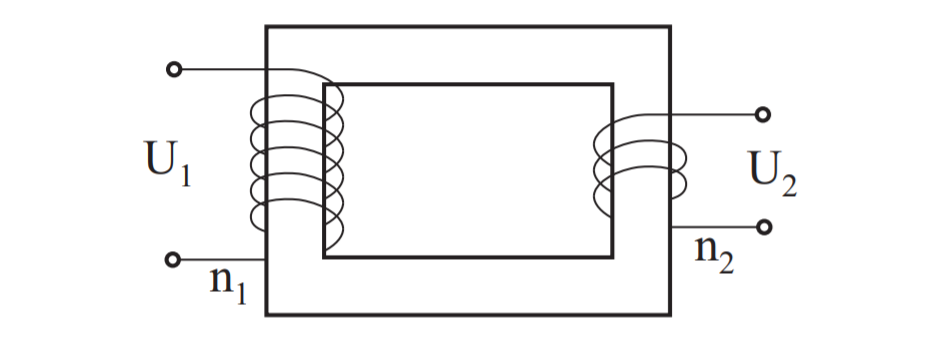
\includegraphics[scale=0.4]{transformator.png}
%~
%}
%\end{figure}

%\newcommand{\R_eins}{R1 $ =(12.00\pm0.12)~\Omega$}
\newcommand{\ifequals}[3]{\ifthenelse{\equal{#1}{#2}}{#3}{}}
\newcommand{\case}[2]{#1 #2} 
\newenvironment{switch}[1]{\renewcommand{\case}{\ifequals{#1}}}{}


\newcommand{\R}[1]{
\begin{switch}{#1}
\case{1}{R1 $ =(1794 \pm 18)~\Omega$}%
\case{2}{R2 $ =(1195 \pm 12)~\Omega$}%
\case{3}{R3 $ =(676.6\pm 6.8)~\Omega$}%
\case{4}{R4 $ =(330.36\pm3.30)~\Omega$}%
\case{5}{R5 $ =(179.8\pm1.8)~\Omega$ }%
\case{6}{R6 $ =(100.40 \pm 1.00 )~\Omega$}%
\case{7}{R7 $ =(68.40 \pm 0.68)~\Omega$}%
\case{8}{R8 $ =(47.60\pm 0.47)~\Omega$ }%
\case{9}{R9 $ =(33.30 \pm 0.33)~\Omega$}%
\case{10}{R10 $ =(12.38\pm 0.12)~\Omega$}%
\case{11}{R11 $ =(18.32\pm 0.18)~\Omega$}%
\end{switch}}

\section{Geräteliste}

\begin{table}[H]
\caption{Liste der verwendeten Geräte}

~

\begin{tabular}{l|p{3cm}p{3.5cm}llll}
Abk. & Typ    & Daten & Inv.Nr.  \\
\hline
O & Oszilloskop  DSO-X 2022A \\
FG1 & Frequenzgenerator  BK precision 4063 &   \\
K1 & Koaxialkabel 1  & $\ell_1=(0.50\pm 0.01)~$m \\
K2 & Koaxialkabel 2  & $\ell_2=(31.20\pm 0.01)~$m \\
 R1 & Widerstand &  \R1 \\
R2 & Widerstand & \R2 \\
R3 & Widerstand & \R3 \\
R4 & Widerstand & \R4 \\
R5 & Widerstand & \R5 \\
R6 & Widerstand & \R6 \\
R7 & Widerstand & \R7 \\
R8 & Widerstand & \R8 \\
R9 & Widerstand & \R9 \\
R10 & Widerstand & \R{10} \\
R11 & Widerstand & \R{11}
\end{tabular}
\end{table}






\section{Beschreibung der Versuchsanordnung}

Im ersten Teil wird der zeitliche Spannungsverlauf am Anfang und Ende des Kabels gemessen. Dabei variiert der Innenwiderstand der Signalquelle. Die Abbildungen \ref{fig:anordnung_task1a}, \ref{fig:anordnung_task1b} und \ref{fig:anordnung_task1c} beschreiben den Aufbau.


\begin{figure}[H]
\centering
\caption{Versuch 1 (a): Signalquelle (FG1) ist mit dem zu testenden Koaxialkabel verbunden. CH1 des Oszilloskops misst den Spannungsverlauf am Anfang des Kabels und CH2 am Ende.}
\label{fig:anordnung_task1a}
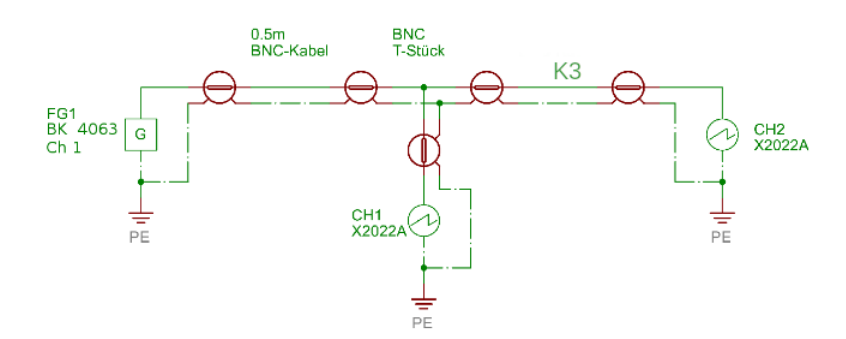
\includegraphics[scale=1.6]{task1a.png}
\end{figure}


\begin{figure}[H]
\centering
\caption{Versuch 1 (a) als Foto. Die Kurven am Oszilloskop zeigen die Daten aus Grafik~\ref{fig:task1a_100ns}.}
\label{fig:foto_task1a}
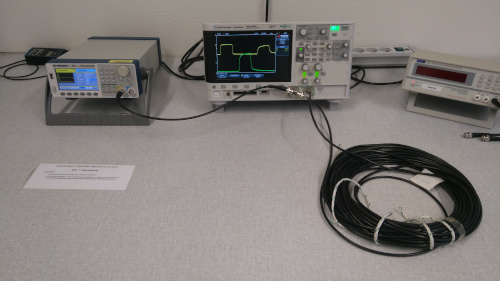
\includegraphics[scale=0.6]{foto_task1a.jpg}
\end{figure}



\begin{figure}[H]
\centering
\caption{Versuch 1 (b): Signalquelle (FG1) ist mit dem zu testenden Koaxialkabel verbunden. Erhöhung des Innenwiderstandes von FG1 durch in Serie geschalteten Widerstand. CH1 des Oszilloskops misst den Spannungsverlauf am Anfang des Kabels und CH2 am Ende.}
\label{fig:anordnung_task1b}
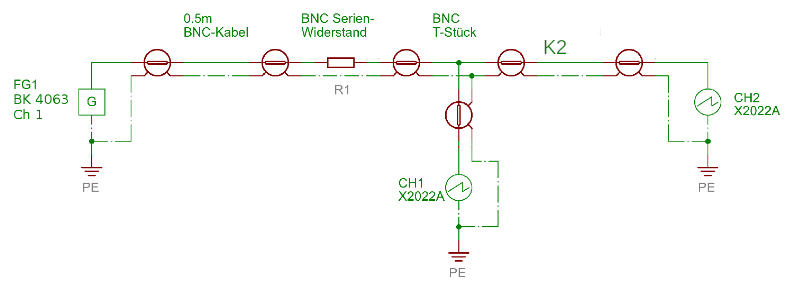
\includegraphics[scale=2]{task1b.png}
\end{figure}



\begin{figure}[H]
\centering
\caption{Versuch 1 (b) als Foto. Die Kurven am Oszilloskop zeigen die Daten aus Grafik \ref{fig:task1b_2300ns}.}
\label{fig:foto_task1b}
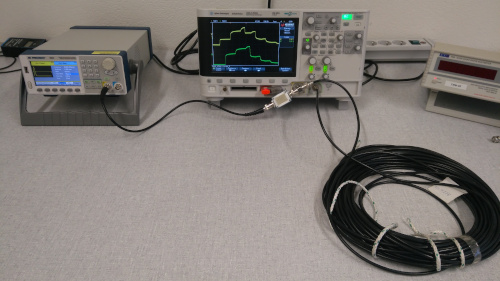
\includegraphics[scale=0.6]{foto_task1b.jpg}
\end{figure}



\begin{figure}[H]
\centering
\caption{Versuch 1 (c): Signalquelle (FG1) ist mit dem zu testenden Koaxialkabel verbunden. Senkung des Innenwiderstandes von FG1 durch parallel geschalteten Widerstand. CH1 des Oszilloskops misst den Spannungsverlauf am Anfang des Kabels und CH2 am Ende.}
\label{fig:anordnung_task1c}
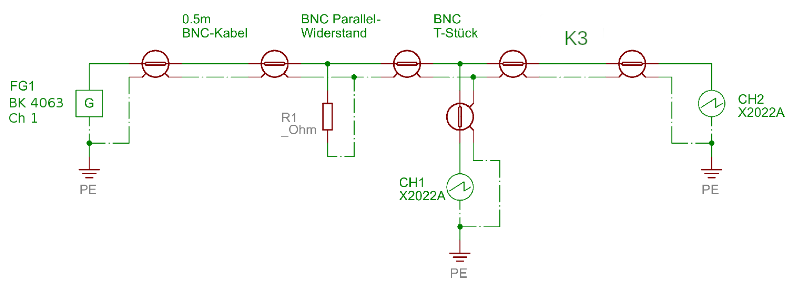
\includegraphics[scale=2]{task1c.png}
\end{figure}



\begin{figure}[H]
\centering
\caption{Versuch 1 (c) als Foto. Die Kurven am Oszilloskop zeigen die Daten aus Grafik \ref{fig:task1c_150ns}.}
\label{fig:foto_task1c}
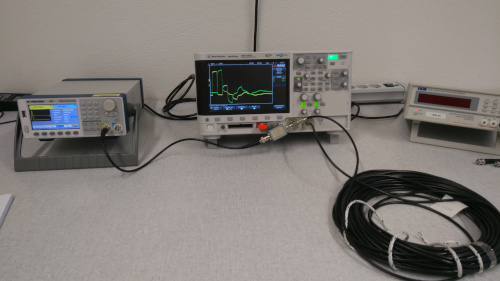
\includegraphics[scale=0.6]{foto_task1c.jpg}
\end{figure}


\begin{figure}[H]
\centering
\caption{Versuch 2: Signalquelle (FG1) ist mit dem zu testenden Koaxialkabel verbunden. CH1 des Oszilloskops misst den Spannungsverlauf am Anfang des Kabels. Am Ende des Kabels befindet sich ein Widerstand. Durch diesen Aufbau kann der Reflexionskoeffizient gemessen werden.}
\label{fig:anordnung_task2}
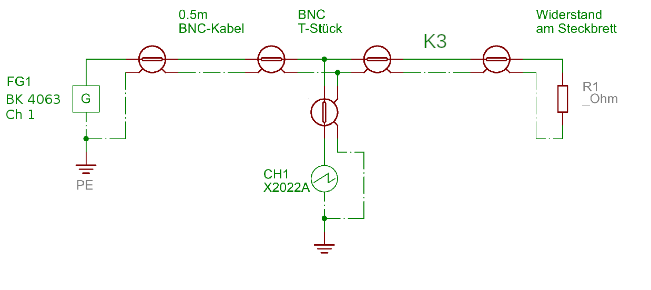
\includegraphics[scale=2]{task2.png}
\end{figure}


Weiters sind in diesem Versuch die Widerstände an einem symmetrischen Verzweiger zu bestimmen. Aus der Theorie ist bekannt, wann der Gesamtwiderstand der Kabelimpedanz $Z_K$ entspricht. Es gilt also nach Grafik~\ref{fig:anordnung_task4}
\begin{align}
\label{eq:verzweiger}
Z_K &= R + (R+50~\Omega)||(R+50~\Omega) = R + \frac{R+50}{2} = \frac{3\cdot R + 50}{2}
\end{align}
Also ist ein symmetrischer Verzweiger gemäß der Aufgabenstellung genau dann störungsfrei, wenn Gleichung~\eqref{eq:verzweiger} gilt.

\begin{figure}[H]
\centering
\caption{Versuch 4: Aufbau eines symmetrischen Verzweigers. $R$ ist so zu wählen, dass keine Reflexionen auftreten.}
\label{fig:anordnung_task4}
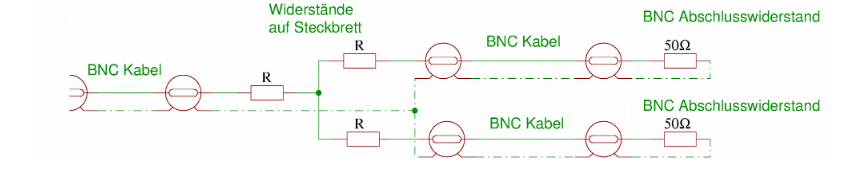
\includegraphics[scale=2]{task4.png}
\end{figure}



\begin{figure}[H]
\centering
\caption{Versuch 4 als Foto. Die Schaltung am Steckbrett entspricht der schematischen Darstellung in Grafik~\ref{fig:anordnung_task4}.}
\label{fig:foto_task4_richtig}
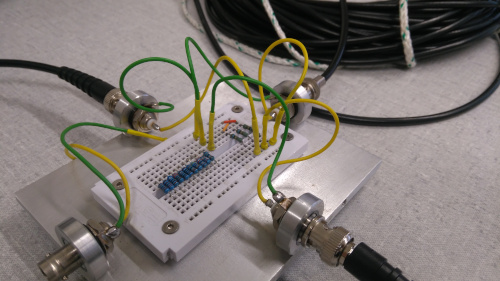
\includegraphics[scale=0.6]{task4_richtig.jpg}
\end{figure}

\begin{figure}[H]
\centering
\caption{Versuch 4 als Foto. Die Schaltung entspricht nicht Grafik~\ref{fig:anordnung_task4}, da die Widerstände in Serie zum Innenleiter (gelbe Drähte) geschaltet werden. Die Außenleiter (grüne Drähte) sind ohne Widerstände verbunden.}
\label{fig:foto_task4_falsch}
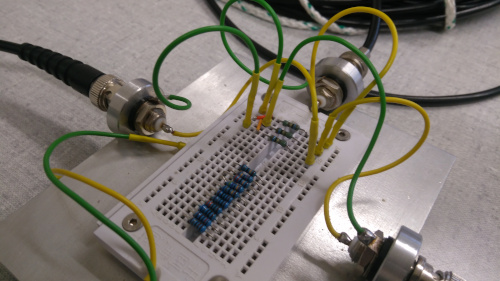
\includegraphics[scale=0.6]{task4_falsch.jpg}
\end{figure}


\section{Versuchsdurchführung und Messwerte}

\subsection{Zeitlicher Spannungsverlauf an den Enden des Koaxialkabels}

\subsubsection{Angepasster Innenwiderstand}

Der Versuchsaufbau ist in Abbildung~\ref{fig:anordnung_task1a} beschrieben bzw. in Abbildung~\ref{fig:foto_task1a} als Foto dargestellt. Der Frequenzgenerator wird auf \texttt{Pulse} mit einer Frequenz von 30~kHz eingestellt. Zusätzlich wird \texttt{PulseWidth} auf $100~$ns, $240~$ns, $500~$ns und $750~$ns gesetzt.



\begin{figure}[H]
\centering
\caption{Spannungsverlauf an beiden Enden des Koaxialkabels mit $t_p=100$~ns.}
\label{fig:task1a_100ns}
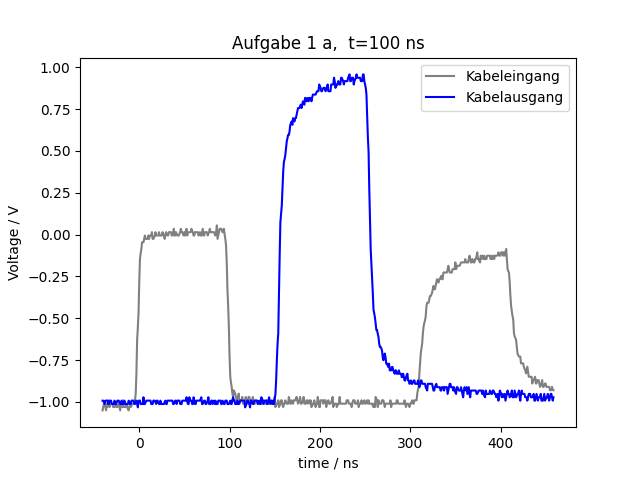
\includegraphics[scale=0.6]{bilder/task1a/task1a_100ns.png}
\end{figure}

\begin{figure}[H]
\centering
\caption{Spannungsverlauf an beiden Enden des Koaxialkabels mit $t_p=240$~ns.}
\label{fig:task1a_240ns}
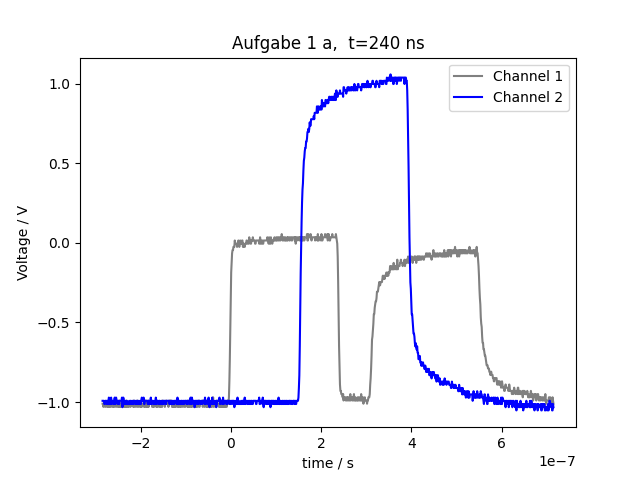
\includegraphics[scale=0.6]{bilder/task1a/task1a_240ns.png}
\end{figure}

\begin{figure}[H]
\centering
\caption{Spannungsverlauf an beiden Enden des Koaxialkabels mit $t_p=500$~ns.}
\label{fig:task1a_500ns}
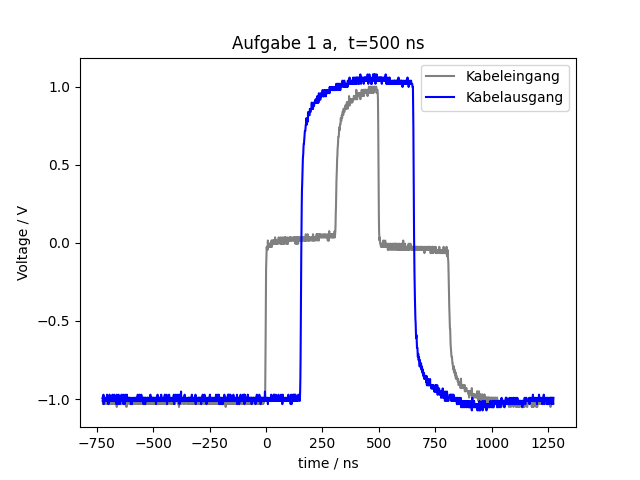
\includegraphics[scale=0.6]{bilder/task1a/task1a_500ns.png}
\end{figure}

\begin{figure}[H]
\centering
\caption{Spannungsverlauf an beiden Enden des Koaxialkabels mit $t_p=750$~ns.}
\label{fig:task1a_750ns}
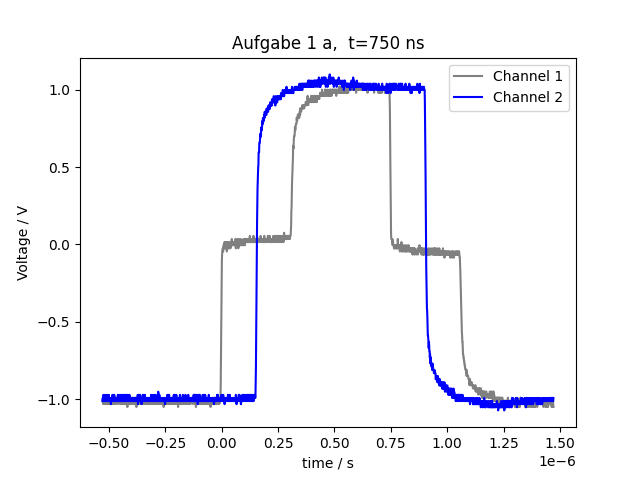
\includegraphics[scale=0.6]{bilder/task1a/task1a_750ns.png}
\end{figure}





\subsubsection{Hoher Innenwiderstand}
Der Versuchsaufbau ist in Abbildung~\ref{fig:anordnung_task1b} beschrieben. Hier soll ein Puls $t_p = 150~$ns und einmal $t_p = 2.3~\mu$s  als Signal verwendet werden.


\begin{figure}[H]
\centering
\caption{Spannungsverlauf an beiden Enden des Koaxialkabels. Hoher Innenwiderstand der Signalquelle. Channel 1 ist Spannung am Beginn des Kabels, Channel 2 am Ende. $t_p = 150~$ns.}
\label{fig:task1b_150ns}
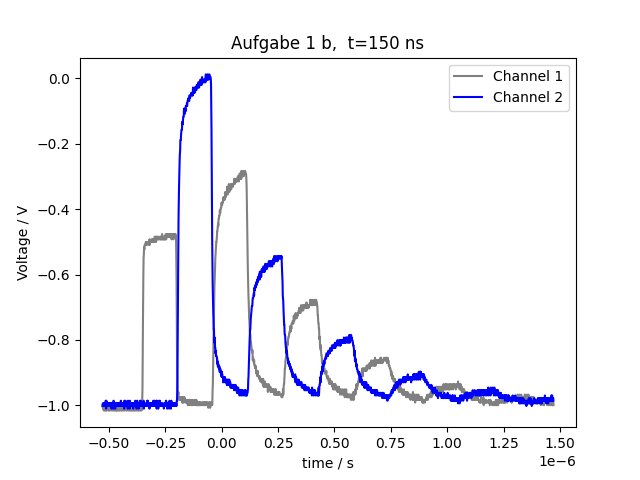
\includegraphics[scale=0.6]{bilder/task1b/task1b_150ns.png}
\end{figure}

\begin{figure}[H]
\centering
\caption{Spannungsverlauf an beiden Enden des Koaxialkabels. Hoher Innenwiderstand der Signalquelle. Channel 1 ist Spannung am Beginn des Kabels, Channel 2 am Ende. $t_p = 2.3~\mu$s.}
\label{fig:task1b_2300ns}
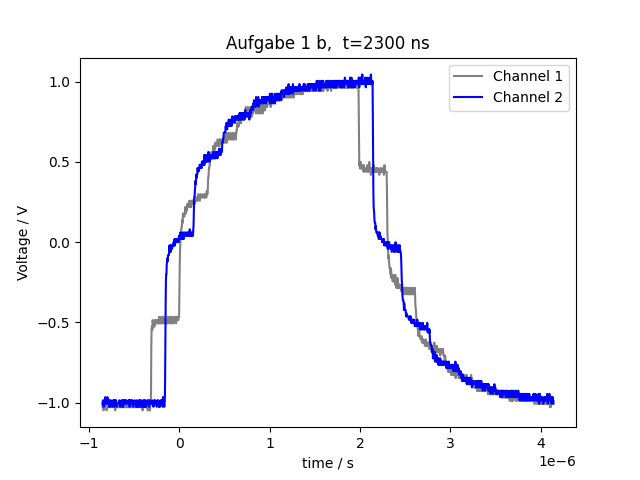
\includegraphics[scale=0.6]{bilder/task1b/task1b_2300ns.png}
\end{figure}



\subsubsection{Niedriger Innenwiderstand}
Der Versuchsaufbau ist in Abbildung~\ref{fig:anordnung_task1c} beschrieben. Hier soll ein Puls $t_p = 150~$ns und einmal $t_p = 2.65~\mu$s  als Signal verwendet werden.

\begin{figure}[H]
\centering
\caption{Spannungsverlauf an beiden Enden des Koaxialkabels. Niedriger Innenwiderstand der Signalquelle. Channel 1 ist Spannung am Beginn des Kabels, Channel 2 am Ende. $t_p = 150$ns.}
\label{fig:task1c_150ns}
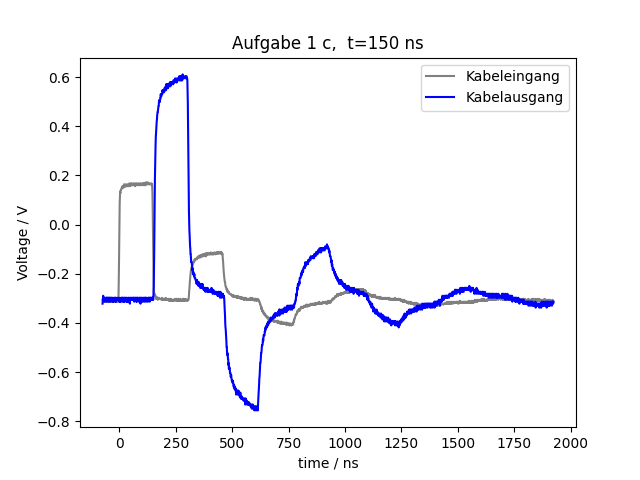
\includegraphics[scale=0.6]{bilder/task1c/task1c_150ns.png}
\end{figure}

\begin{figure}[H]
\centering
\caption{Spannungsverlauf an beiden Enden des Koaxialkabels. Niedriger Innenwiderstand der Signalquelle. Channel 1 ist Spannung am Beginn des Kabels, Channel 2 am Ende. $t_p = 2.65~\mu$s.}
\label{fig:task1b_2650ns}
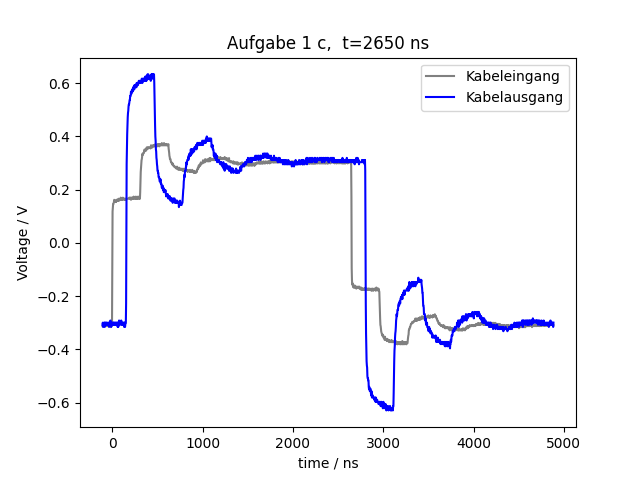
\includegraphics[scale=0.6]{bilder/task1c/task1c_2650ns.png}
\end{figure}



\subsection{Bestimmung des Reflexionskoeffizienten und der Kabelimpedanz}

Der Versuchsaufbau ist in Grafik~\ref{fig:anordnung_task2} beschrieben.

Die Frequenz wurde auf 30~kHz gestellt und die Pulszeit $t_p = 200~$ns. Jetzt stehen 11 verschiedene Widerstände zur Verfügung (siehe Geräteliste), welche jeweils als Abschlusswiderstand des Kabels genutzt werden. Diese Widerstände werden hier nochmal in einer Tabelle zusammengefasst.

Einige dieser Widerstände wurden mehrmals gemessen. In diesem Fall wird der Mittelwert herangezogen bzw. die Standardabweichung auf die 10\%-ige Unsicherheit addiert (sofern signifikant). Diese Widerstände sind der Vollständigkeit halber auch in der Geräteliste zusammengefasst.

\begin{table}[H]
\centering
\caption{Widerstände für diesen Versuch.}
\begin{tabular}{l|l}
Bezeichnung & Wert \\
\hline
R1 & \R1 \\
R2 & \R2 \\
R3 & \R3 \\
R4 & \R4 \\
R5 & \R5 \\
R6 & \R6 \\
R7 & \R7 \\
R8 & \R8 \\
R9 & \R9 \\
R10 & \R10 \\
R11 & \R11 
\end{tabular}

\end{table}

Im Gegensatz zu Aufgabe 1 wird hier nur die Eingangsspannung gemessen. Der Eingangswiderstand der Signalquelle ist angepasst, so wie in 1 (a). Am Ende des Kabels werden verschiedene Widerstände angeschlossen. Der Spannungsverlauf dieser Widerstände wird in den Grafiken~\ref{fig:task2_R1} bis \ref{fig:task2_kurz} dargestellt.


\begin{figure}[H]
\centering
\caption{Spannungsverlauf am Kabeleingang. Am Kabelausgang befindet sich der Widerstand \R1}
\label{fig:task2_R1}
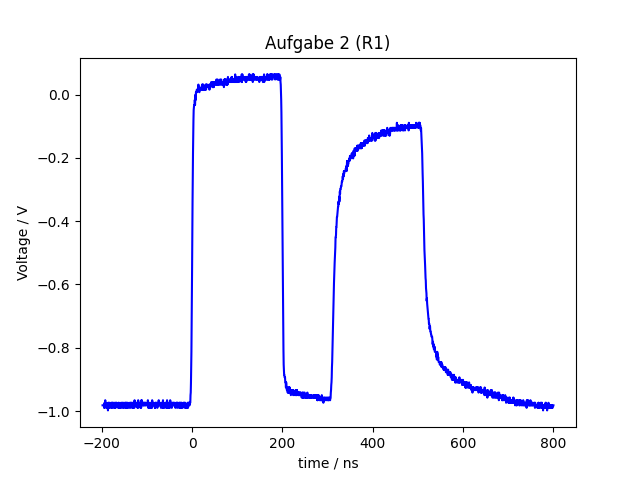
\includegraphics[scale=0.6]{bilder/task2/task2_R1.png}
\end{figure}



\begin{figure}[H]
\centering
\caption{Spannungsverlauf am Kabeleingang. Am Kabelausgang befindet sich der Widerstand \R2}
\label{fig:task2_R2}
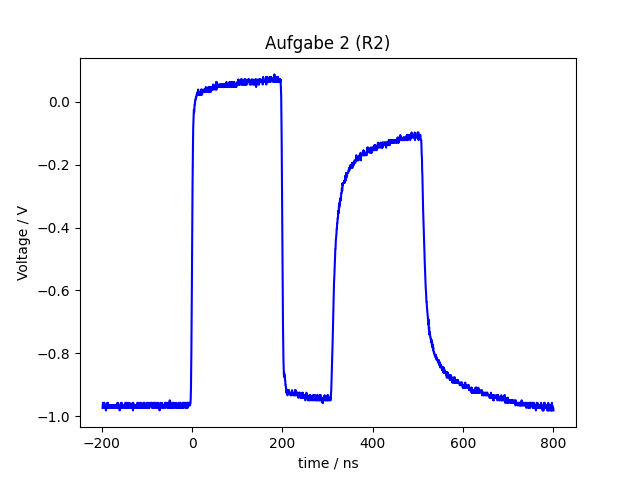
\includegraphics[scale=0.6]{bilder/task2/task2_R2.png}
\end{figure}



\begin{figure}[H]
\centering
\caption{Spannungsverlauf am Kabeleingang. Am Kabelausgang befindet sich der Widerstand \R3}
\label{fig:task2_R3}
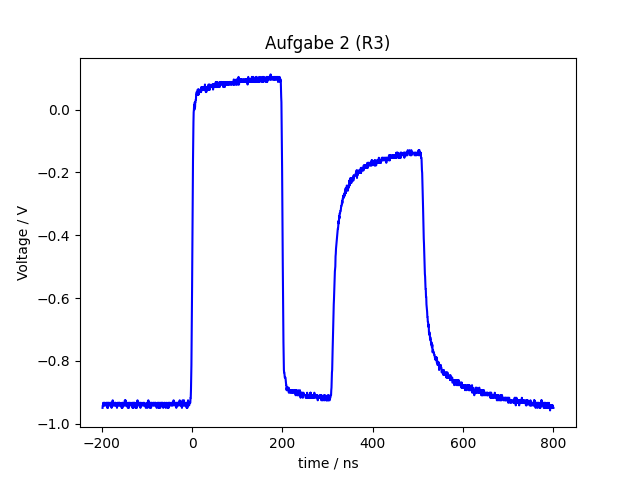
\includegraphics[scale=0.6]{bilder/task2/task2_R3.png}
\end{figure}


\begin{figure}[H]
\centering
\caption{Spannungsverlauf am Kabeleingang. Am Kabelausgang befindet sich der Widerstand \R4}
\label{fig:task2_R4}
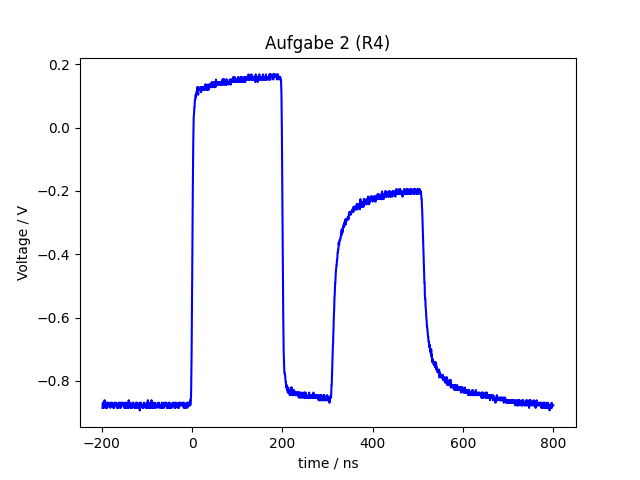
\includegraphics[scale=0.6]{bilder/task2/task2_R4.png}
\end{figure}




\begin{figure}[H]
\centering
\caption{Spannungsverlauf am Kabeleingang. Am Kabelausgang befindet sich der Widerstand \R5}
\label{fig:task2_R5}
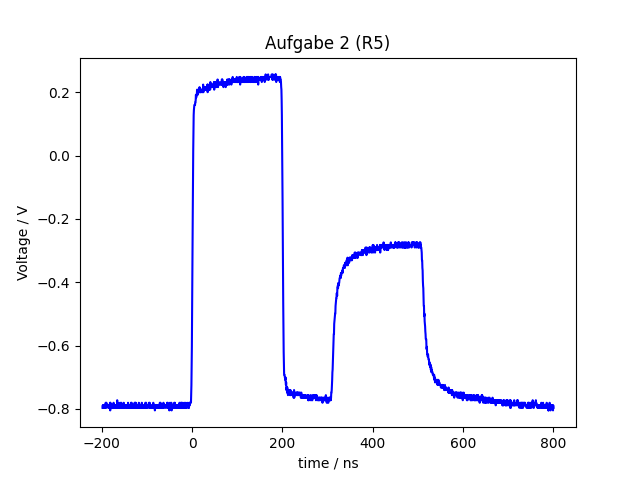
\includegraphics[scale=0.6]{bilder/task2/task2_R5.png}
\end{figure}



\begin{figure}[H]
\centering
\caption{Spannungsverlauf am Kabeleingang. Am Kabelausgang befindet sich der Widerstand \R6}
\label{fig:task2_R6}
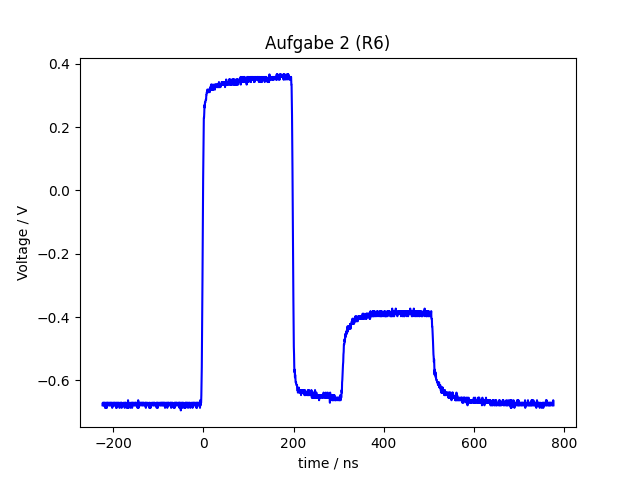
\includegraphics[scale=0.6]{bilder/task2/task2_R6.png}
\end{figure}




\begin{figure}[H]
\centering
\caption{Spannungsverlauf am Kabeleingang. Am Kabelausgang befindet sich der Widerstand \R7}
\label{fig:task2_R7}
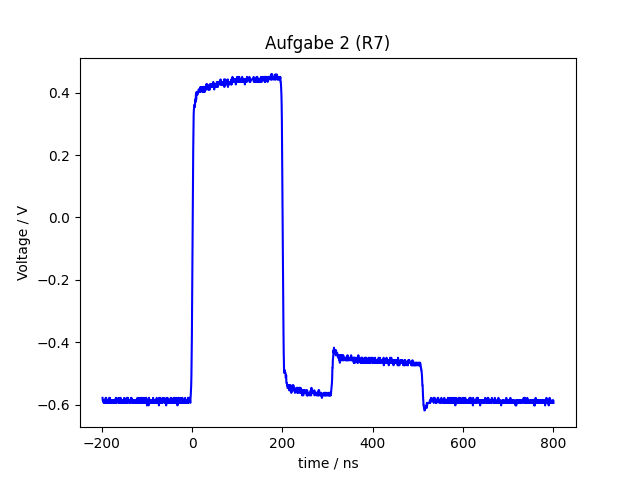
\includegraphics[scale=0.6]{bilder/task2/task2_R7.png}
\end{figure}





\begin{figure}[H]
\centering
\caption{Spannungsverlauf am Kabeleingang. Am Kabelausgang befindet sich der Widerstand \R8}
\label{fig:task2_R8}
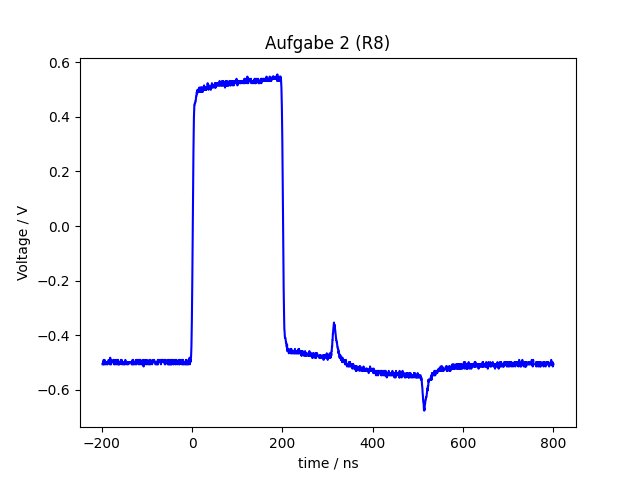
\includegraphics[scale=0.6]{bilder/task2/task2_R8.png}
\end{figure}




\begin{figure}[H]
\centering
\caption{Spannungsverlauf am Kabeleingang. Am Kabelausgang befindet sich der Widerstand \R9}
\label{fig:task2_R9}
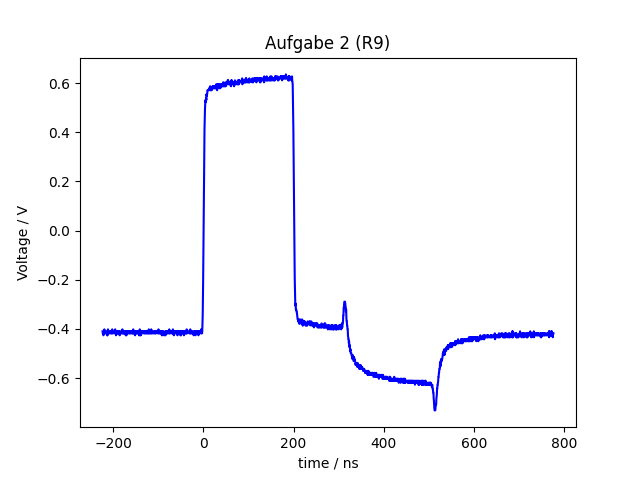
\includegraphics[scale=0.6]{bilder/task2/task2_R9.png}
\end{figure}





\begin{figure}[H]
\centering
\caption{Spannungsverlauf am Kabeleingang. Am Kabelausgang befindet sich der Widerstand \R{10}}
\label{fig:task2_R10}
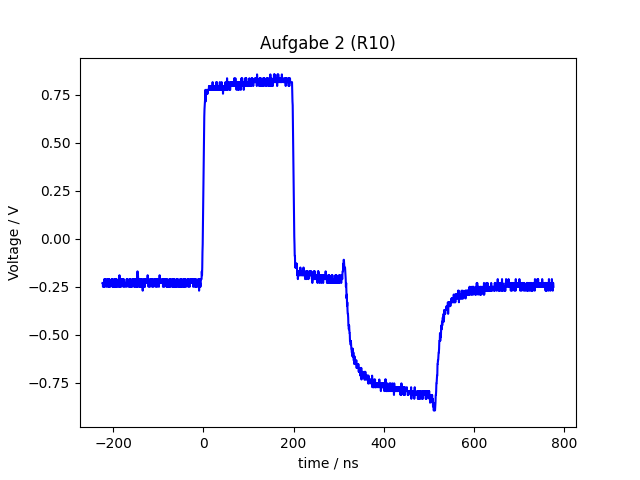
\includegraphics[scale=0.6]{bilder/task2/task2_R10.png}
\end{figure}



\begin{figure}[H]
\centering
\caption{Spannungsverlauf am Kabeleingang. Am Kabelausgang befindet sich der Widerstand \R{11}}
\label{fig:task2_R11}
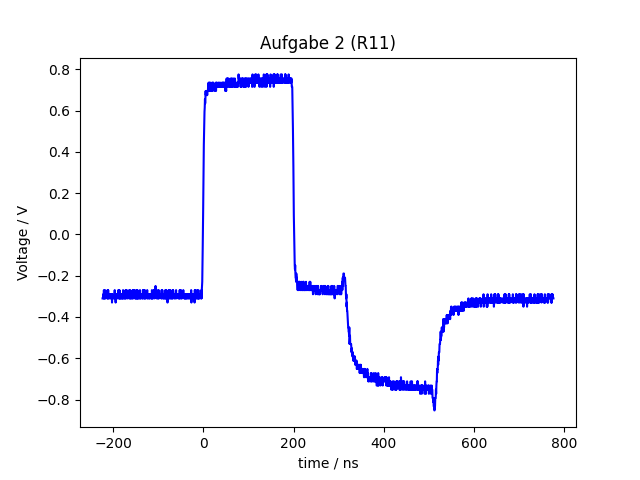
\includegraphics[scale=0.6]{bilder/task2/task2_R11.png}
\end{figure}


\begin{figure}[H]
\centering
\caption{Spannungsverlauf am Kabeleingang. Am Kabelausgang befindet sich ein Kurzschluss}
\label{fig:task2_kurz}
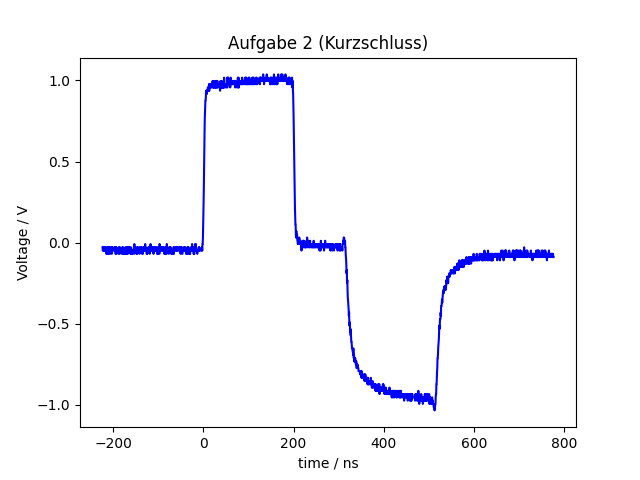
\includegraphics[scale=0.6]{bilder/task2/task2_kurz.png}
\end{figure}




\subsection{Bestimmung der Signalgeschwindigkeit}

Hierbei wird ein Puls augesendet und jene Zeit gemessen, bis der reflektierte Impuls gemessen wird. Es eignen sich dafür die Signale mit $t_p=100~$ns und $t_p=240~$ns aus Aufgabe 1 (a). Die Zeitmessung ist in den Grafiken~\ref{fig:task3_100ns} und \ref{fig:task3_240ns} veranschaulicht.

Die abgelesenen Zeiten werden in Tabelle~\ref{tab:task3_zeiten} dargestellt.
\begin{table}[H]
\caption{Zeitpunkt von einem Puls $t_1$ bis zu dessen Reflexion $t_2$. Das Ablesen erfolgt händisch aus den Daten an jenem Punkt, wo die Spannung die Schwelle von -0.8~V übersteigt. Wegen des Rauschens ist die Unsicherheit von $t_1,t_2$ jeweils 5~ns und $\Delta \tau = 10~$ns.}
\label{tab:task3_zeiten}
\begin{tabular}{l|lll}
$t_p$ / ns & $t_1$ / ns & $t_2$ / ns & $\tau$ / ns  \\
\hline
100 &  -3.13 & 310.16 & 313.29 \\
240 &  -3.38 & 308.63 & 312.01
\end{tabular}
\end{table}

\begin{figure}[H]
\centering
\caption{Zeitmessung (grün) bei einem Signal mit einer Pulsdauer von 100~ns.}
\label{fig:task3_100ns}
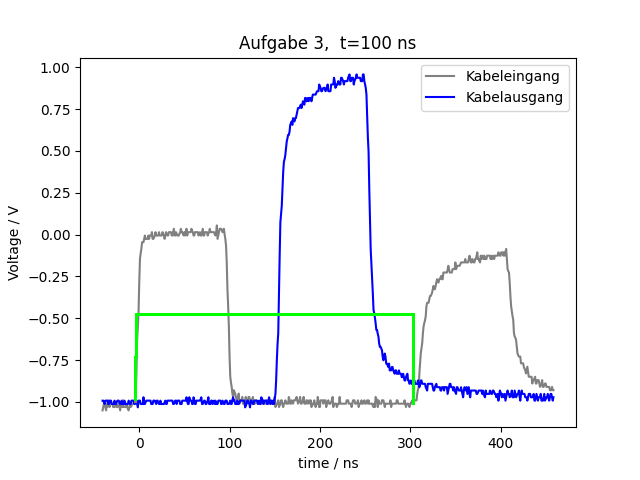
\includegraphics[scale=0.6]{bilder/task3/task3_100ns.png}
\end{figure}

\begin{figure}[H]
\centering
\caption{Zeitmessung (grün) bei einem Signal mit einer Pulsdauer von 240~ns.}
\label{fig:task3_240ns}
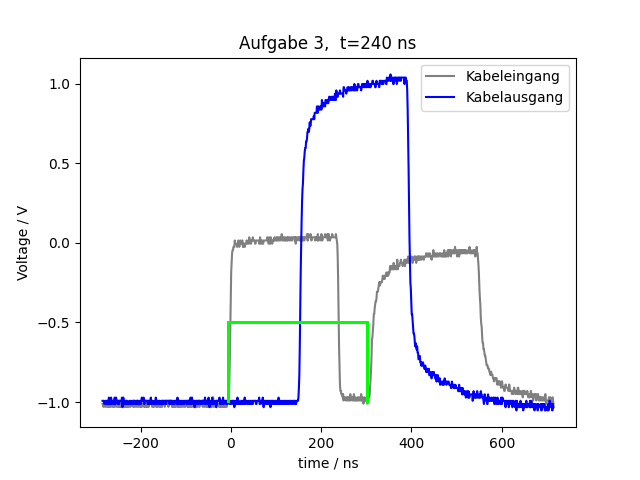
\includegraphics[scale=0.6]{bilder/task3/task3_240ns.png}
\end{figure}


\subsection{Wiederstände an einem symmetrischen Verzweiger}

In Grafiken~\ref{fig:foto_task4_richtig} und \ref{fig:foto_task4_falsch} ist die Schaltung eines symmetrischen Verzweigers dargestellt. Grafik~\ref{fig:foto_task4_richtig} zeigt den korrekten Aufbau des Verzweigers. Der im Foto verwendete Widerstand hat die Farbkombination \textit{braun-blau-schwarz-gold-braun}. Wegen COVID-19 ist die Messung der Reflexion an einem symmetrischen Verzweiger momentan nicht möglich.


\section{Auswertung}

\subsection{Zeitlicher Spannungsverlauf an den Enden des Koaxialkabels}

\subsubsection{Angepasster Innenwiderstand}
Die Grafiken \ref{fig:task1a_100ns} bis \ref{fig:task1a_750ns} beschreiben den Spannungsverlauf am Anfang und am Ende des Kabels mit angepassten Widerstand. Nachdem das Signal durch das Kabel läuft, wird es am Ende reflektiert, da es sich um ein offenes Ende handelt. Das Signal in die eine Richtung überlagert sich mit dem Signal aus der entgegen gesetzten Richtung und es entsteht Interferenz. Durch den angepassten Innenwiderstand in der Signalquelle wird das Signal dort nicht reflektiert. Daher legt das Signal den Weg durch das Kabel zwei mal zurück (vom Anfang zum Ende, und retour).

Am Kabelausgang wird das Signal bei der Reflexion mit sich selbst überlagert, daher ist am Kabelausgang eine Verdoppelung der Spannung zu erkennen.

Dies lässt sich am Beispiel von~\ref{fig:task1a_100ns} zeigen. Von 0~ns bis 100~ns wird der erste Puls gesendet. Dieser wird bei 170~ns bis 270~ns am Kabelausgang gemessen. Danach wird er zwischen 310~ns und 410~ns wieder am Kabeleingang gemessen. Man erkennt deutlich, dass der Puls bei der Reflexion am Kabelausgang seine Rechtecksform verliert. Das reflektierte Signal am Kabeleingang hat eine ähnliche Form wie bei der Interferenz am Kabelende.


Grafik~\ref{fig:task1a_240ns} ist ähnlich wie Grafik~\ref{fig:task1a_100ns}. Durch den längeren Puls ist der zeitliche Abstand des Eingangssignals mit dem reflektierten Signal deutlich geringer. Bei einer weiteren Erhöhung der Pulsdauer ist eine Überlagerung am Signaleingang zu erwarten.

In Grafik~\ref{fig:task1a_500ns} tritt genau diese Überlagerung auf. Die beiden Rechteckspulse werden teilweise überlagert und es kommt zur Verdoppelung der Spannung an der Überlappung der beiden Signale.

Mit Steigerung der Pulsdauer steigt die Überlappung der Signale. Grafik~\ref{fig:task1a_750ns} zeigt das deutlich. Für sehr lange Pulsdauern wäre die Verzögerung durch das Kabel vernachlässigbar und man würde am Kabeleingang die doppelte Spannung sehen.


\subsubsection{Hoher Innenwiderstand}

Durch den hohen Innenwiderstand ist am Anfang des Kabels eine Reflexion zu beobachten. Durch die stärkere Reflexion sieht man, dass eine \textit{Treppenfunktion} entsteht, da sich die Signale mehrfach im Kabel hin und her bewegen und sich ständig überlagern. Da die Höhe der Treppen immer kleiner wird, lässt sich darauf schließen, dass das Signal bei mehrmaligem Vor- und Zurücklauf kontinuierlich abgeschwächt wird.

Grafik~\ref{fig:task1b_150ns} ist ein Sonderfall. Wie schon in Grafik~\ref{fig:task1a_100ns} zu sehen ist, benötigt das Signal durch das Kabel circa 150~ns. Da die Pulsdauer auf genau diese Zeit eingestellt ist, lässt sich eine gewisse Periodizität erkennen. Zu Beginn wird ein Puls der Länge 150~ns gesendet. Dieser wird eben nach 150~ns am Kabelausgang mit doppelter Spannung (wegen Interferenz) gemessen und wieder zum Kabelanfang reflektiert. 150~ns später wird er am Kabeleingang gemessen und erneut reflektiert. Damit wird der Puls abwechselnd am Kabeleingang und Kabelausgang gemessen, während die Amplitude durch den Widerstand in jeder Periode abnimmt.

Grafik~\ref{fig:task1b_2300ns} hingegen zeigt einen Puls, der deutlich länger ist als 150~ns. Es wird ein Puls durch das Kabel gesendet, ca. 150~ns später wird er in doppelter Höhe am Kabelausgang reflektiert. Weitere 150~ns später gelangt das Signal wieder an den Kabeleingang, wo allerdings noch die Spannung des Pulses anliegt. Daher wird am Kabeleingang das reflektierte Signal mit dem immer noch andauernden Puls überlagert und erhöht sich entsprechend. Dieser Vorgang wird mehrmals wiederholt, wobei das reflektierte Signal sich durch den Widerstand abschwächt, sodass die Sprünge in der Treppenfunktion immer geringer werden. 


\subsubsection{Niedriger Innenwiderstand}

Durch die Senkung des Widerstandes im Kabelanschluss, sinkt die Anschlussimpedanz $Z_A$ unter jene der Kabelimpedanz $Z_K$. Wegen $Z_A < Z_K$ ist der Reflexionskoeffizient negativ und es folgt $\rho < 0$ wegen Gleichung~\eqref{eq:reflexionskoeff}. Damit wird die Spannung bei der Reflexion umgekehrt.

Grafik~\ref{fig:task1c_150ns} zeigt diesen Fall für 150~ns Pulsdauer. Während der erste Eingangspuls und dessen Reflexion am Ausgang noch deutlich zu erkennen ist, wird der Ausgangspuls am Kabelanfang ins negative umgekehrt, was sich aber durch den reflektierten Impuls aufhebt. Durch die Pulsdauer von 150~ns sieht man alle 150~ns einen Sprung.

\subsection{Bestimmung des Reflexionskoeffizienten und der Kabelimpedanz}

Zu Beginn muss die Eingangsspannung $U_e$ und die reflektierte Spannung $U_r$ gemessen werden. in Tabelle~\ref{tab:reflexionskoeff} sind die jeweiligen Werte dargestellt. Zusätzlich wurde der Reflexionskoeffizient berechnet. Der Reflexionskoeffizient kann auf zwei verschiedene Arten bestimmt werden, nämlich mit den Formeln~\eqref{eq:reflexionskoeff1} und \eqref{eq:reflexionskoeff}. Für die nachfolgende Tabelle wird Formel \eqref{eq:reflexionskoeff1} verwendet.

\begin{table}[H]
\centering
\caption{Bestimmung der Eingangs- und Ausgangsspannung für alle Widerstände R1 bis R11 und für einen Kurzschluss. Zusätzlich wurde der Reflexionskoeffizient $\rho$ und dessen Unsicherheit berechnet. Wegen dem Rauschen wird eine Unsicherheit $\Delta U_e = \Delta U_r = 30~$mV angenommen.}
\label{tab:reflexionskoeff}
\begin{tabular}{c|llll}
Widerstand Nr. & $U_e$ / mV & $U_r$ / mV & $\rho$ / 1 & $\Delta \rho$ / 1 \\
\hline
R1 & 1020 & 874 & 0.86 & 0.05 \\
R2 & 1026 & 848 & 0.82 & 0.05 \\
R3 & 1026 & 781 & 0.76 & 0.05 \\
R4 & 1026 & 668 & 0.65 & 0.05 \\
R5 & 1023 & 505 & 0.49 & 0.04 \\
R6 & 1024 & 287 & 0.28 & 0.04 \\
R7 & 1026 & 127 & 0.12 & 0.03 \\
R8 & 1025 & -30 & -0.03 & 0.03 \\
R9 & 1022 & -181 & -0.17 & 0.02 \\
R10 & 1038 & -533 & -0.51 & 0.01\\
R11 & 1034 & -415 & -0.40 & 0.02 \\
Kurzschluss & 1037 & -445 & -0.43 & 0.02
\end{tabular}
\end{table}


Nach Formel~\eqref{eq:reflexionskoeff} gibt es einen Zusammenhang zwischen dem Ausgangswiderstand, der Kabelimpedanz und den Reflexionskoeffizienten
\begin{align*}
\rho = \frac{Z_A-Z_K}{Z_A+Z_K}
\end{align*}
wobei für $Z_A$ die Widerstände aus Tabelle~\ref{tab:reflexionskoeff} eingesetzt werden können. Insbesondere jene Werte von R7 und R8 sind von Interesse, da sich genau an dieser Stelle das Vorzeichen ändert. Es folgt, dass die Kabelimpedanz nahe bei 50~$\Omega$ liegen muss, da bei $R_8 = 47.60~\Omega$ der Reflexionskoeffizient am nähesten bei $0$ liegt.

Durch lineare Interpolation ergibt sich
\begin{align}
\label{eq:interpolation}
0 \approx \rho\left(\text{R8} + \frac{\text{R7}-\text{R8}}{\rho(\text{R7}) - \rho(\text{R8})} \cdot \big(0 -\rho(\text{R8}) \big)  \right) = \rho\left(\left(51.76 \pm 56.85\right)~\Omega\right)
\end{align}

Diese Unsicherheit ist sehr groß im Vergleich zum Messwert. Das liegt daran, dass der Nenner in Gleichung~\eqref{eq:interpolation} den Term $\rho(\text{R7}) - \rho(\text{R8})$ enthält und dieser sehr klein wird (0.15). Der Zähler ist die Differenz aus R7 und R8 und entsprechend größer (20.8~$\Omega$). Gemäß den Unsicherheiten ergibt sich eine hohe numerische Instabilität. Es kann in diesem Fall dennoch davon ausgegangen werden, dass $Z_K \approx 50~\Omega$ ist, da dieser ein für BNC Kabel üblicher Wert ist (vgl. \cite{bnc}). Für genauere Analysen wären mehrere Messwerte wichtig. 


Der Vollständigkiet halber wurden die Spannungskurven der verschiedenen Widerstände nochmal alle in Grafik~\ref{fig:task2_summary} zusammengefasst, wobei die Eingangsspannung normiert wurde. Die Unterscheidung der Kurven erfolgt nach dem Kriterium, ob der jeweilige Abschlusswiderstand größer oder kleiner als die Kabelimpedanz ist. Es ist hier sehr leicht zu erkennen, dass die Kabelimpedanz zwischen den Werten der Widerstände R7 und R8 liegen muss. Diese sind in der gegebenen Grafik grau markiert. Man erkennt hier, dass dort am wenigsten Reflexion auftritt. Außerdem erkennt man, dass die Eingangsspannung in allen Fällen circa gleich groß ist. 

\begin{figure}[H]
\centering
\caption{Spannungsverlauf am Kabeleingang von allen Widerständen gegenübergestellt. Dazu wurde zu den Spannungen ein jeweiliges Offset addiert. Die blauen Kurven gehören zu jenen Widerständen, die größer sind als die Kabelimpedanz. Die orangen Kurven sind zu den Widerständen die kleiner sind als die Kabelimpedanz. Die beiden grauen Kurven gehören zu den Widerständen R7 und R8.}
\label{fig:task2_summary}
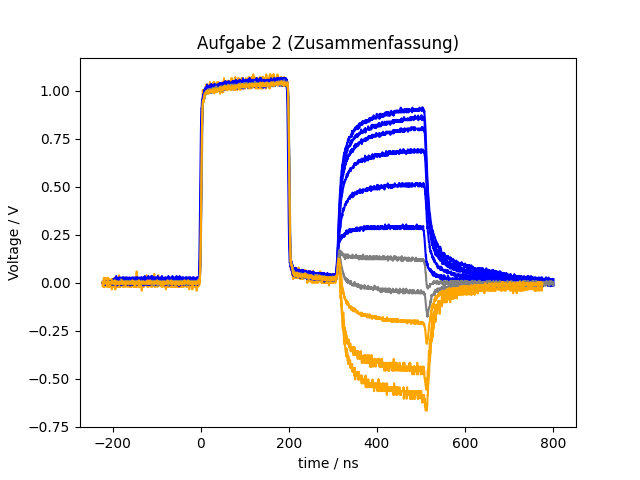
\includegraphics[scale=0.6]{bilder/task2/task2_summary.png}
\end{figure}



\subsection{Bestimmung der Signalgeschwindigkeit}

Der elektrische Impuls legt den Weg $s = 2\cdot \ell_2$ zurück. Wenn dafür die Zeit $\tau$ benötigt wird, dann gilt insgesamt mit Größtfehlermethode
\begin{align*}
c = \left(\frac{2\cdot \ell_2}{\tau} \pm \left|\frac{2\cdot \Delta \ell_2}{\tau} + \frac{2\cdot \ell_2}{\tau^2}\cdot \Delta \tau\right|\right)
\end{align*}
Man setzt $\tau = 312.65~$ns (Mittelwert aus Tabelle~\ref{tab:task3_zeiten}) und $\Delta \tau = 10~$ns. Aus der Geräteliste kann man $\ell_2 = (31.20 \pm 0.01)~$m ablesen. Daraus folgt
\begin{align*}
c = \left(200 \pm  6\right)\cdot 10^6~\text{m/s}
\end{align*}

Die relative Permittivität des Isoliermaterials ist hier außerdem zu berechnen. Aus $\varepsilon \cdot \mu = \frac{1}{c^2}$ folgt inklusive Fehleranalyse
\begin{align*}
\varepsilon_r = \frac{1}{c^2\cdot \mu\cdot \varepsilon_0} \pm \left| \frac{\Delta c}{c^3\cdot \mu\cdot \varepsilon_0} \right|
\end{align*}
mit der elektrischen Feldkonstanten $\varepsilon_0$, der magnetischen Feldkonstanten $\mu_0$, sowie $\mu = \mu_r\cdot\mu_0$ und $\mu_r=1$. Daraus folgt
\begin{align*}
\varepsilon_r = 2.26 \pm 0.07
\end{align*}


\subsection{Wiederstände an einem symmetrischen Verzweiger}

Aus Gleichung~\eqref{eq:verzweiger} geht folgende Gleichung hervor, dass folgendes gilt
\begin{align*}
Z_K = \frac{3\cdot R + 50~\Omega}{2}
\end{align*}
Für $Z_K = (51.76\pm56.85)~\Omega$ ergibt sich
\begin{align*}
R = (17.84 \pm 37.9)~\Omega
\end{align*}
Auch hier ist die Unsicherheit relativ hoch. Dies resultiert aus der Unsicherheit der Kabelimpedanz.

Am dazugehörigen Foto ist der Widerstand gezeigt. Die darauf zu sehenden Farben sind \textit{braun-blau-schwarz-gold-braun}. Das lässt sich gemäß \cite{resistor} auf 16~$\Omega$ mit einer Toleranz von 1\% zurückführen. Aufgrund der großen Unsicherheit kann man hier leider keine seriösen Schlüsse ziehen.




\section{Diskussion}


\subsection{Zeitlicher Spannungsverlauf an den Enden eines Koaxialkabels}

Die Spannungsverläufe an den Enden des Koaxialkabels verhalten sich wie es in der Theorie vorhergesagt wird. 


\subsection{Bestimmung des Reflexionskoeffizienten und der Kabelimpedanz}

Die Kabelimpedanz wird mit Hilfe von linearer Interpolation bestimmt, was aber problematisch ist. Erstens ist der Zusammenhang in seiner Gesamtheit nicht linear und wird nur an einer Stelle linear approximiert, andererseits erhält man durch die Skalierung der Achsen eine gewisse numerische Instabilität. Zusätzlich werden die nötigen Größen aus einem rauschenden Signal gemessen. Trotz Mittelung zur Reduktion des Rauschens muss eine gewisse Unsicherheit angenommen werden.



\subsection{Bestimmung der Signalgeschwindigkeit}

Die Relativitätstheorie besagt, dass die Geschwindigkeits stets kleiner als die Vakuumlichtgeschwindigkeit sein muss. Tatsächlich beträgt die Signalgeschwindigkeit 2/3 der Vakuumlichtgeschwindigkeit. Dieses Ergebnis ist als sehr verlässlich einzustufen, da erstens die Unsicherheit entsprechend niedrig ist, und zweitens die Zeitmessung in einem Oszilloskop im Vergleich zur Messung der Spannung genau ist. Auch das Rauschen stellt hier kein Problem dar.

\subsection{Wiederstände an einem symmetrischen Verzweiger}

Gleichung~\eqref{eq:verzweiger} kann für $Z_K = 50~\Omega$ umgeschrieben werden
\begin{align*}
50 = \frac{3\cdot R + 50}{2}
\end{align*}
Daraus ergibt sich $R = \dfrac{50}{3} = 16.67~\Omega$, was vom berechneten Wert von $17.84~\Omega$ etwas abweicht. Im Versuchsaufbau wurde ein 16~$\Omega$ Widerstand verwendet. Im Experiment wird der ideale Wert vermutlich unter dem berechneten Wert liegen, da die Kabel selbst auch einen Innenwiderstand besitzen. Dieser müsste entsprechend zu dem seriell geschalteten Widerstand addiert werden.


\section{Zusammenfassung}

Zuerst wurden Pulse verschiedener Länge durchs Kabel gesendet. Die Spannung wurde an beiden Enden des Kabels gemessen. Am Kabelende war die Spannung verdoppelt, das das Signal und das reflektierte Signal sich überlagern. Da die Impedanz am Signalgenerator dem Kabel angepasst ist, gab es keine mehrfache Reflexion. Bei Erhöhung des Innenwiderstandes des Signalgenerators konnte eine Reflexion beobachtet werden. Dadurch wurde das Signal mehrfach überlagert. Bei Verringerung des Widerstandes im Funktionsgenerator wurde der Reflexions\-koeffizient negativ und kann daher eine Umkehr der Spannung messen.

~

Die Kabelimpedanz $Z_K$ wird versuchsweise durch Variation des Endwiderstandes bestimmt. Es zeigt sich, dass die geringste Reflexion bei \R8 auftritt. Durch lineare Interpolation ergibt sich $Z_K \approx 51~\Omega$, allerdings mit einer zu hohen Abweichung.

~

Die Signalgeschwindigkeit im Kabel liegt bei $c = (200 \pm 6)\cdot 10^6~$m/s, was ca 2/3 der Vakuumlichtgeschwindigkeit entspricht.

~

Für die Widerstände im symmetrischen Verzweiger ergibt sich laut Theorie $R=16.67~\Omega$, nach der Rechnung ergeben sich $17.84~\Omega$, welche aber eine starke Unsicherheit aufgrund der Kabelimpedanz haben. In der Praxis wird man aber einen deutlich niedrigeren Wert einsetzen, da das Kabel selbst auch einen Widerstand hat. Am Foto des Versuchsaufbaus ist ein Widerstand $R=16~\Omega \pm 1\%$ zu erkennen.

%\newpage 
%\appendix
%\section{Python Skript}



\definecolor{commentgreen}{RGB}{2,112,10}
\definecolor{eminence}{RGB}{108,48,130}
\definecolor{weborange}{RGB}{255,165,0}
\definecolor{frenchplum}{RGB}{129,20,83}

\lstdefinelanguage{python}{
    morekeywords={def, for, range, abs, return},
    otherkeywords={<-,->, |>, \%\{, \}, \{, \, (, )},
    sensitive=true,
    morecomment=[l]{\#},
    morecomment=[n]{/*}{*/},
    morecomment=[s][\color{purple}]{:}{\ },
    morestring=[s][\color{orange}]"",
    commentstyle=\color{commentgreen},
    keywordstyle=\color{eminence},
    stringstyle=\color{red},
	basicstyle=\ttfamily,
	breaklines,
	showstringspaces=false,
	frame=tb
}
%\lstinputlisting[language=Python,captionpos=b, label=lst:test,caption={Python Skript}]{generate_numbers.py}

%\lstinputlisting[language=Python,captionpos=b, label=lst:test,caption={Bessel Auswertung}]{generate_numbers_bessel.py}


%\lstinputlisting[language=Python,captionpos=b, label=lst:test,caption={Zerstreuungslinse Auswertung}]{generate_numbers_zerstreuungslinse.py}


\begin{thebibliography}{9}
\bibitem{moodle} Unterlagen aus Moodle, A. Hohenau, bereitgestellt von der KF Universität Graz.
\bibitem{bnc} \url{https://de.wikipedia.org/wiki/BNC-Steckverbinder}, aberufen am 24.11.2020, 15:00.
\bibitem{resistor} \url{https://www.conrad.de/de/ratgeber/technik-einfach-erklaert/widerstands-farbcode.html}, abgerufen am 24.11.2020, 15:00.
\end{thebibliography}


\end{document}
